\documentclass[report.tex]{subfiles}
\begin{document}
\section{Baseline without Middleware (75 pts)}\label{exp2}

This section establishes a performance baseline of the \emph{memtier benchmark} clients and \emph{memcached} servers in the cloud.

\subsection{One Server}\label{exp21}

%Both, for a read-only and write-only workload plot the throughput and the response time as a function of NumClients. All clients are connected to a single memcached instance.

%Use 3 load generating VMs, with one memtier (CT=2) each, and vary the number of virtual clients (VC) per memtier thread between 1 and 32. Show how the behavior of the server changes as we add more clients.

In this set of experiments the behaviour of the system with 3 load generating VMs and 1 server VM is analysed. The detailed experiment configuration is presented in the table below.


\begin{center}
	\scriptsize{
		\begin{tabular}{|l|c|}
			\multicolumn{2}{l}{3 client VMs and 1 server VM}\\
			%\hline Number of servers                & 1                        \\ 
			%\hline Number of client machines        & 3                        \\ 
			\hline Instances of memtier per machine & 1                        \\ 
			\hline Threads per memtier instance     & 2                        \\
			\hline Virtual clients per thread       & [1, 2, 4, 8, 12, 16, 24, 32]\\ 
			\hline Workload                         & Write-only and Read-only \\
			%\hline Multi-Get behavior               & N/A                      \\
			%\hline Multi-Get size                   & N/A                      \\
			%\hline Number of middlewares            & N/A                      \\
			%\hline Worker threads per middleware    & N/A                      \\
			%\hline Repetitions                      & 3 (at least 1 minute each)\\ 
			\hline 
		\end{tabular}
	}
\end{center}

Apart from the client measurements for throughput and response time, the graphs also contain the throughput and response time derived from the interactive law\footnote{the interactive law $R = \frac{N}{X} - Z$ shows the relationship between response time $R$ and throughput $X$ in a closed system with $N$ clients and a client thinking time of $Z$} with a client thinking time of $Z=0$ and a maximal achievable throughput due to the network bandwidth limit between the VMs when using values of size 4096B.

\begin{figure}[H]
\begin{subfigure}{\linewidth}
	\begin{subfigure}[b]{.49\linewidth}
		\centering
		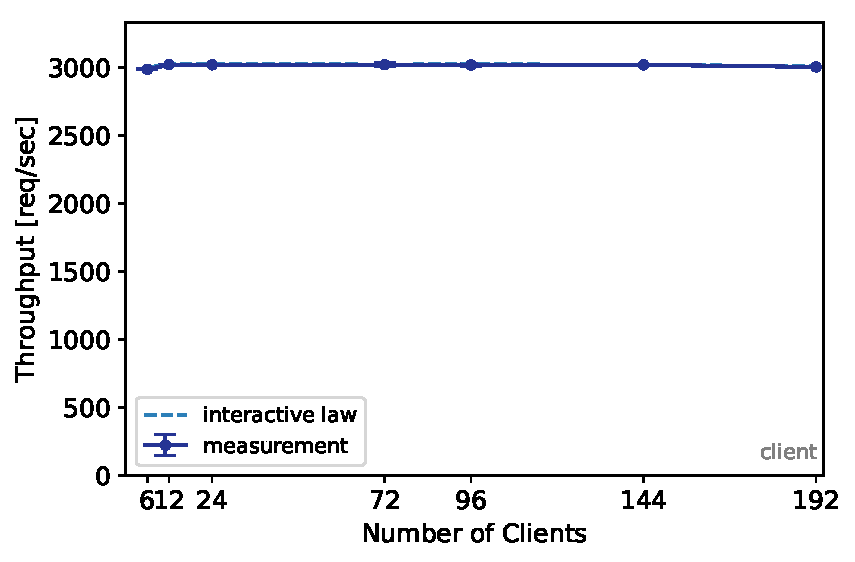
\includegraphics[width=\linewidth]{data/exp21_ro_tp_nc.pdf}
	\end{subfigure}\hfill
	\begin{subfigure}[b]{.49\linewidth}
		\centering
		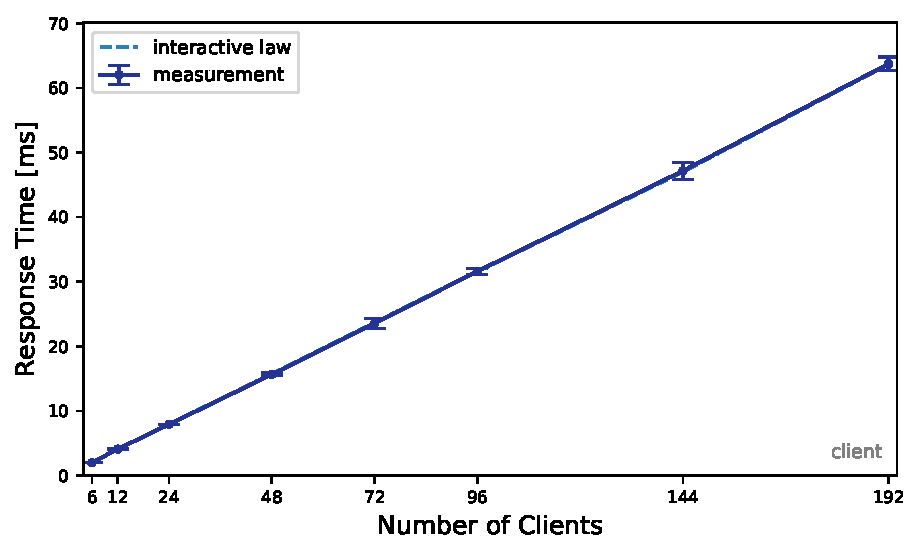
\includegraphics[width=\linewidth]{data/exp21_ro_rt_nc.pdf}
	\end{subfigure}%
	\caption{read-only workload}
	\label{exp21_ro_nc}
\end{subfigure}
\\[1ex]
\begin{subfigure}{\linewidth}
	\begin{subfigure}[b]{.49\linewidth}
		\centering
		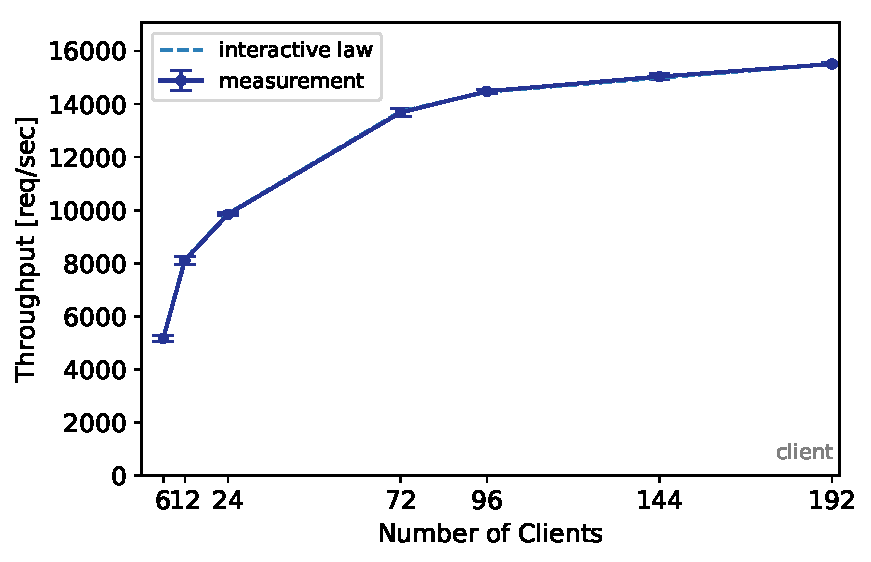
\includegraphics[width=\linewidth]{data/exp21_wo_tp_nc.pdf}
	\end{subfigure}\hfill
	\begin{subfigure}[b]{.49\linewidth}
		\centering
		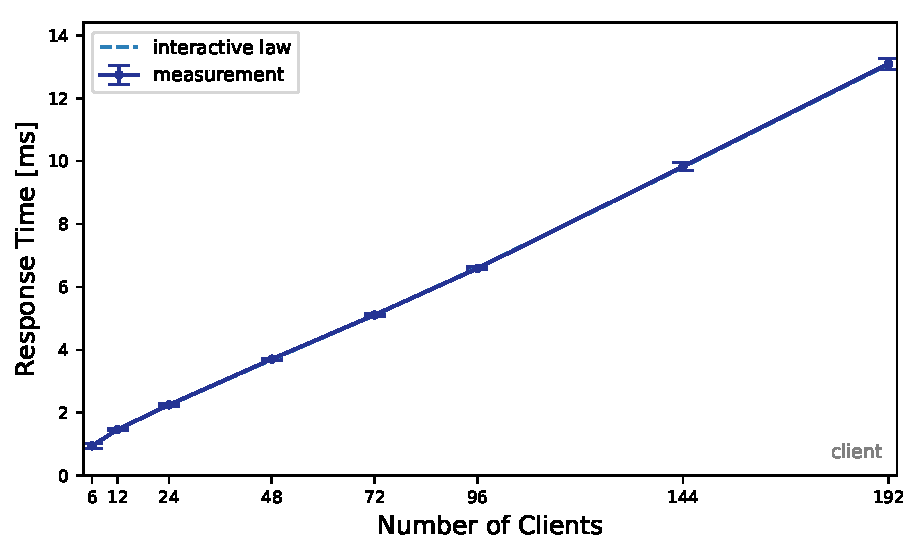
\includegraphics[width=\linewidth]{data/exp21_wo_rt_nc.pdf}
	\end{subfigure}%
	\caption{write-only workload}
	\label{exp21_wo_nc}
\end{subfigure}
\caption{Throughput and response time measurements of the system with one server verified with the interactive law as a function of the number of clients. The error metric is the sample standard deviation over the repetitions and the maximal throughput due to the network bandwidth is shown.}
\end{figure}



\subsubsection{Explanation}

\paragraph{Read-Only Workload}
As shown in figure \ref{exp21_ro_nc}, the throughput saturation for the read-only workload is already reached at 6 clients because the upload bandwidth of the single server VM limits the throughput. The server VM upload bandwidth was measured to be 99.6 MBit/sec. When using a value size of 4096B, this results in a maximum possible throughput of 3040 ops/sec for a read-only workload because all values need to be sent from the server VM to one of the 3 client VMs. 
Consequently increasing the number of clients has almost no effect on the throughput while the response time grows linearly because more clients result in more requests on the server that need to wait to be sent through the bottleneck to a client VM.

\paragraph{Write-Only Workload}
In figure \ref{exp21_wo_nc} it can be observed that for a write-only workload the throughput saturation is reached at 72 clients. In this experiment the bottleneck is not the bandwidth but rather the \emph{memcached} server. 
As expected the throughput first increases in the number of clients while the \emph{memcached} servers are still under-saturated. The response time of the \emph{memcached} server does not show the typical behaviour between the under-saturated and saturated phase, because even though the throughput still increases drastically, the response time is already showing a linear increase without a clear knee.
However, even though using 96 clients would result in a marginally higher throughput, the increase in response time does not justify a user load of more than 72 clients as the maximum throughput and hence with more than 72 clients the system is saturated. The over-saturated phase with decreasing throughput is not shown because \emph{memcached} is able to keep the throughput stable even for a large user-load.


\subsection{Two Servers}\label{exp22}


This set of experiments analyses the behaviour of the system with 1 load generating VM and two server VMs. The detailed experiment configuration is presented in the table below.

\begin{center}
	\scriptsize{
		\begin{tabular}{|l|c|}
			\multicolumn{2}{l}{1 client VM and 2 server VMs}\\
			%\hline Number of servers                & 2                        \\ 
			%\hline Number of client machines        & 1                        \\ 
			\hline Instances of memtier per machine & 2                        \\ 
			\hline Threads per memtier instance     & 1                        \\
			\hline Virtual clients per thread       & [1, 2, 4, 8, 12, 16, 24, 32]\\ 
			\hline Workload                         & Write-only and Read-only \\
			%\hline Multi-Get behavior               & N/A                      \\
			%\hline Multi-Get size                   & N/A                      \\
			%\hline Number of middlewares            & N/A                      \\
			%\hline Worker threads per middleware    & N/A                      \\
			%\hline Repetitions                      & 3 (at least 1 minute each) \\ 
			\hline 
		\end{tabular}
	} 
\end{center}

As in the previous section, the throughput and response time derived from the interactive law with a client thinking time of $Z=0$ and the network bandwidth limit for the throughput presented next to the measurements obtained from the client.

\begin{figure}[H]
\begin{subfigure}{\linewidth}
	\begin{subfigure}[b]{.49\linewidth}
		\centering
		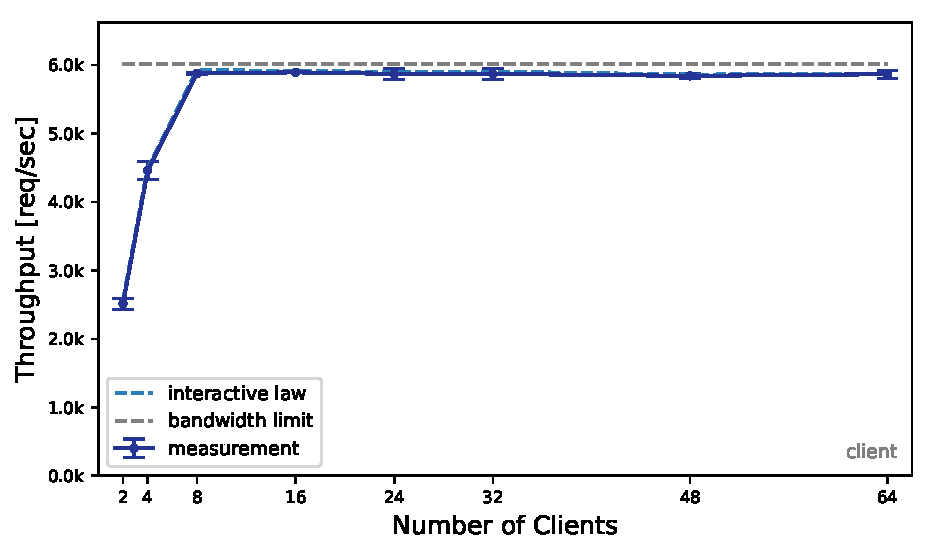
\includegraphics[width=\linewidth]{data/exp22_ro_tp_nc.pdf}
	\end{subfigure}\hfill
	\begin{subfigure}[b]{.49\linewidth}
		\centering
		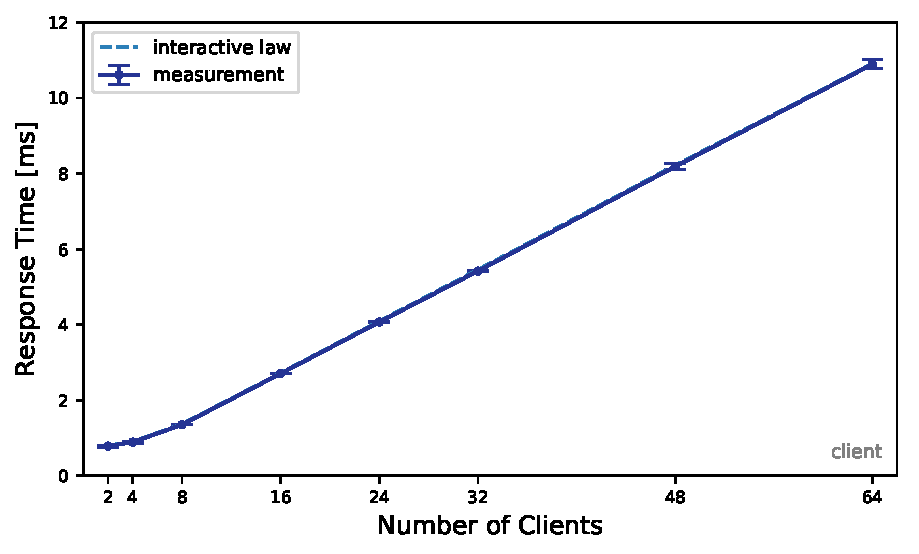
\includegraphics[width=\linewidth]{data/exp22_ro_rt_nc.pdf}
	\end{subfigure}%
	\caption{read-only workload}
	\label{exp22_ro_nc}
\end{subfigure}
\\[1ex]
\begin{subfigure}{\linewidth}
	\begin{subfigure}[b]{.49\linewidth}
		\centering
		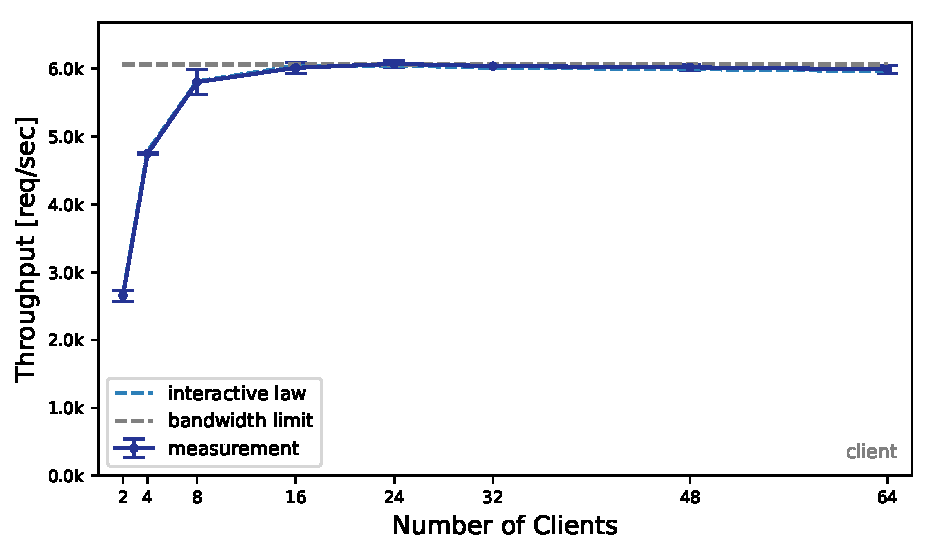
\includegraphics[width=\linewidth]{data/exp22_wo_tp_nc.pdf}
	\end{subfigure}\hfill
	\begin{subfigure}[b]{.49\linewidth}
		\centering
		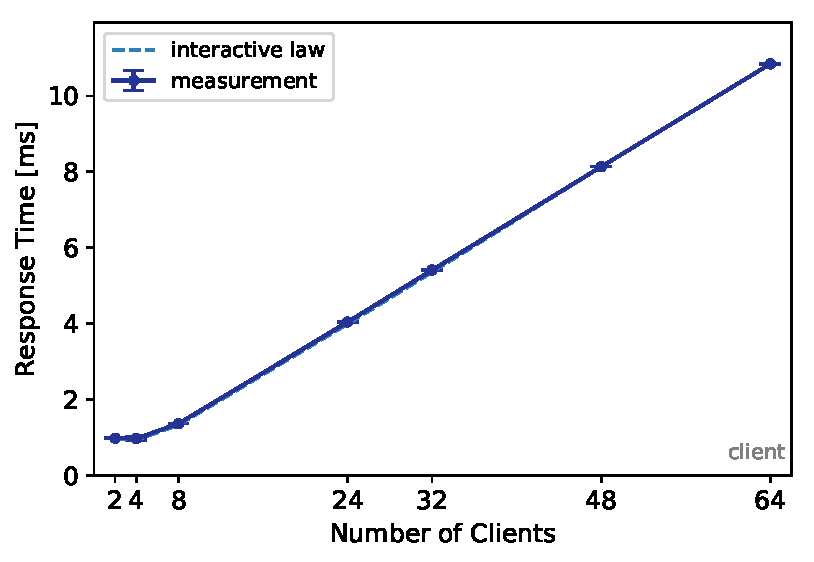
\includegraphics[width=\linewidth]{data/exp22_wo_rt_nc.pdf}
	\end{subfigure}%
	\caption{write-only workload}
	\label{exp22_wo_nc}
\end{subfigure}
\caption{Throughput and response time measurements of the system with one load generating VM verified with the interactive law as a function of the number of clients. The error metric is the sample standard deviation over the repetitions and the maximal throughput due to the network is shown.}
\end{figure}



\subsubsection{Explanation}

\paragraph{Read-Only}
As with a single server VM, the throughput of the read-only workload with 2 servers is also bound by the total upload bandwidth of the server VMs. This becomes evident when considering that two server VMs have a measured total upload bandwidth capacity of 199 MBit/sec which results in an estimate of 6062 ops/sec for the maximally achievable throughput when using values of 4096B.

The optimal number of clients for a read-only workload would be somewhere in between 4 and 8 clients because when using 8 clients the bandwidth bottleneck is already affecting the throughput and response time. However, from the evaluated number of clients it cannot be justified to state that 4 clients is the load with maximum throughput because the increase in throughput of around 1500 ops/sec with 8 clients simply outweights the cost of only 0.45 ms more in response time on average. Consequently the point of throughput saturation is reached at 8 clients. For fewer number of clients the system is under-saturated and for more it is saturated. The over-saturation phase with decreasing throughput is omitted. (Fig. \ref{exp22_ro_nc})


\paragraph{Write-Only}
Using a write-only workload with values of 4096B the situation is similar but here instead of the upload bandwidth of the server VMs, the bottleneck is the upload bandwidth of the load generating client VM. The measured 199 MBit/sec total upload bandwidth limits the throughput of the system to 6062 ops/sec. So as a consequence  the throughput saturation is reached at 8 clients as shown in figure \ref{exp22_wo_nc}. The increase in response time between 4 and 8 clients is still justified for the additional throughput obtained with 8 clients. But the additional 200 ops/sec for 16 clients is not enough to outweigh a response time that is almost twice as long.


\subsection{Summary}


\begin{center}
	{Maximum throughput of different VMs.}
	\begin{tabular}{|l|p{2cm}|p{2cm}|p{4cm}|}
		\hline                        & Read-only workload & Write-only workload & Configuration gives max. throughput \\ 
		\hline One memcached server   & 2962 ops/sec       & 14097 ops/sec & 6 clients for read-only 72 clients for write-only\\ 
		\hline One load generating VM & 5878 ops/sec       &  5802 ops/sec & 8 clients for read-only \hphantom{0} 8 clients for write-only\\ 
		\hline 
	\end{tabular}
\end{center}


%Write at least two paragraphs about how both results relate. Describe what is the bottleneck of this setup is. If the maximum throughput for both experiments is the same, explain why. If it is not the case, explain why not. Write down key take-away messages about the behaviour of the memtier clients and the memcached servers.

\paragraph{Comparison of one memcached server vs. one load generating VM}
For a read-only workload both experiments are bound by the network upload bandwidth of the server VM(s).
Despite the fact that they are both network bound, they have a different maximum throughput because having an additional server in the second set of experiments gives two times the upload bandwidth between server and client VMs and thus resulting in approximately two times the throughput.

The different throughput for write-only workloads is explained by considering that only the second experiment is bound by the network. Namely by the upload bandwidth of the client VM. The bottleneck in the first experiment is \emph{memcached} which saturates for around 72 clients.

\paragraph{Comparison of workloads}
In the first set of experiments with one \emph{memcached} server the throughput is different between write and read workload. 
This is primarily because only the read workload is network bound. For a SET request the server only needs to transmit the 8B confirmation message \texttt{STORED\textbackslash r\textbackslash n} to the client compared to a GET request where the server needs to transport a message with at least 4096B. 

Despite the fact that in the second set of experiments with only one load generating VM the throughput for read-only and write-only is almost identical, the bottleneck is a different part of the system. For read-only it is the upload bandwidth of the two server VMs and for the write-only workload it is the upload bandwidth of the load generating client VM.

\paragraph{Key take-away messages}
\begin{itemize}
	\vitemsep
	\item a single server VM cannot handle more than 3000 ops/sec in a read-only workload
	\item a single client VM cannot simulate a higher write-only workload than 6000 ops/sec
	\item in a write-only workload the point of saturation for 1 server VM is around 14000 ops/sec
\end{itemize}

\end{document}